\chapter{Project Framework}
\label{chap:projectdef}



\begin{wrapfigure}{R}{0.3\textwidth}
	\centering
	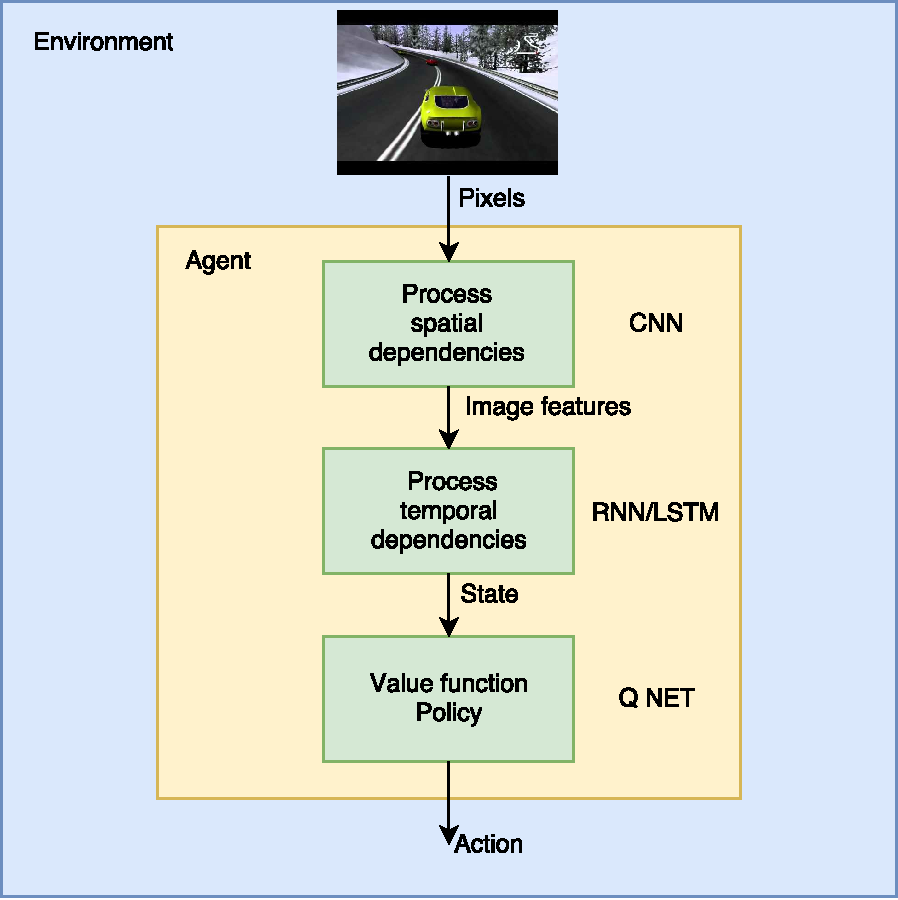
\includegraphics[width=0.6\textwidth]{Figures/ProjectFramework/Project_framework_diagram}
	\caption{The framework for the system used in this project}
	\label{fig:Project_framework}
\end{wrapfigure}
This project is about learning a car or robot to control and navigate it self. This should be done so the robot don't hit walls or obstacles. to solve this problem, a framework is created, the framework can be seen on \Cref{fig:Project_framework}.

The agent takes information from the environment, in this project the information used as input to the agent is an image. The agent uses the pixels from the image, to process spatial dependencies. The spatial dependencies is found by using of convolutional neural networks (CNN). The output from the CNN is the image features. The image features is used to process the temporal dependencies. To find the temporal dependencies a Recurrent Neural Network (RNN) is used. The RNN used is a special RNN called Long Short Term Memory network (LSTM). When both the spatial and temporal dependencies are found, the state the environment is found. This state is used to build the value function and a policy, which is describe a the Q-network. After the value function and the policy is found, the best suited action to the environment can be determined.


The framework is created with inspiration from the papers  \cite{DBLP:journals/corr/MnihBMGLHSK16} and \cite{Sallab:2017:2470-1173:70}
\newline




%\begin{figure}[H]
%	\centering
% 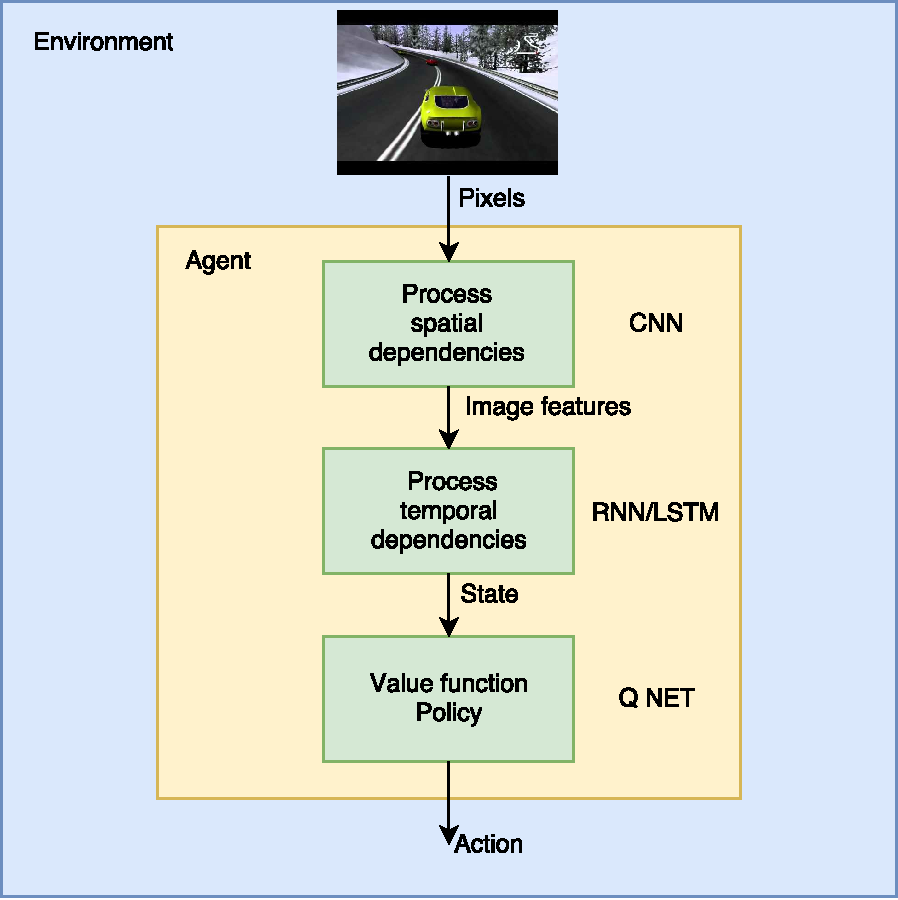
\includegraphics[width=0.3\textwidth]{Figures/ProjectFramework/Project_framework_diagram}
%	\caption{The framework for the system used in this project}
%	\label{fig:Project_framework}
%\end{figure}

\subsubsection*{Convolutional Neural Networks (CNNs)}

Convolutional Neural Networks are similar to normal Neural Networks. They are made up of neurons that have learn able weights and biases. Each neuron receives some inputs, perform a dot product and sometimes follows it with a non-linearity. The whole network expresses a single differentiable score function - from raw image pixels to class scores. CNN architectures make the assumption that the image is, which make it possible to encode certain properties into the architecture. It makes the forward function more efficient to implement and reduce the amount of parameters in the network     

\section{Recurrent Neural Networks}
...
\subsection{Long Short Term Memory}
...